\section{上位の候補地}
\label{sec:sites}

\subsection{候補地の比べ方}

全候補の地図から、互いに \SI{30}{\kilo\metre} 以上離れた上位の地点を、標準と短時間の
飛行のそれぞれで 8 地点ずつ選び、壱岐の 2 地点を加えた 16 地点で、飛行条件の
ばらつき（64 通り）を入れて計算し直した。地点名は最寄りの地名である。

\begin{table}[htbp]
\centering
\scriptsize
\caption{候補地ごとの確率。「落下」は落下予測が目標に入る確率（雪を問わない、標準の飛行）、
「雪なし」は打ち上げ地点に雪がない確率、「地上気象」は 9 時の風・雨が向く確率。
右の 2 列が 4 条件をすべて満たす「実施できる」確率で、括弧内は年ごとのブロック・
ブートストラップによる 95\% 区間。標準の飛行の順に並べた。}
\label{tab:sites}
\resizebox{\linewidth}{!}{\begin{tabular}{lcrrrcc}
\toprule
候補地 & 緯度, 経度 & 落下 & 雪なし & 地上気象 & \multicolumn{2}{c}{実施できる確率 [\%]} \\
& & [\%] & [\%] & [\%] & 標準 (95\% 区間) & 短時間 (95\% 区間) \\
\midrule
平戸・大島 & 33.50, 129.55 & 47 & 99 & 70 & \textbf{33} (30--35) & \textbf{34} (30--37) \\
唐津・加唐島 & 33.60, 129.85 & 44 & 99 & 70 & \textbf{32} (29--35) & \textbf{45} (42--48) \\
下関・蓋井島 & 34.10, 130.80 & 40 & 98 & 77 & \textbf{31} (29--33) & \textbf{36} (34--38) \\
山口・徳地 & 34.25, 131.65 & 41 & 90 & 79 & \textbf{30} (28--33) & \textbf{35} (33--38) \\
壱岐・郷ノ浦 & 33.75, 129.70 & 49 & 98 & 59 & \textbf{30} (27--32) & \textbf{38} (35--42) \\
壱岐（島の中央） & 33.78, 129.72 & 48 & 98 & 59 & \textbf{29} (26--32) & \textbf{38} (35--42) \\
廿日市 & 34.35, 132.30 & 36 & 93 & 83 & \textbf{28} (27--30) & \textbf{43} (40--45) \\
長門・三隅 & 34.35, 131.30 & 40 & 96 & 70 & \textbf{28} (25--30) & \textbf{26} (24--28) \\
佐世保・宇久島 & 33.25, 129.10 & 40 & 99 & 70 & \textbf{27} (25--29) & \textbf{15} (13--17) \\
岩国 & 34.20, 132.00 & 38 & 81 & 81 & \textbf{27} (24--29) & \textbf{31} (28--34) \\
北九州・若松 & 33.90, 130.80 & 35 & 98 & 77 & \textbf{26} (24--28) & \textbf{39} (37--42) \\
糸島・志摩 & 33.60, 130.20 & 35 & 94 & 73 & \textbf{24} (21--28) & \textbf{48} (45--51) \\
唐津・相知 & 33.35, 130.00 & 30 & 99 & 81 & \textbf{23} (20--27) & \textbf{42} (40--45) \\
福津 & 33.75, 130.50 & 33 & 96 & 73 & \textbf{23} (20--26) & \textbf{44} (40--46) \\
東広島 & 34.45, 132.85 & 26 & 87 & 85 & \textbf{20} (18--22) & \textbf{42} (38--45) \\
吉野ヶ里 & 33.35, 130.40 & 20 & 99 & 87 & \textbf{16} (13--19) & \textbf{37} (35--40) \\
\bottomrule
\end{tabular}
}
\end{table}

\begin{figure}[htbp]
\centering
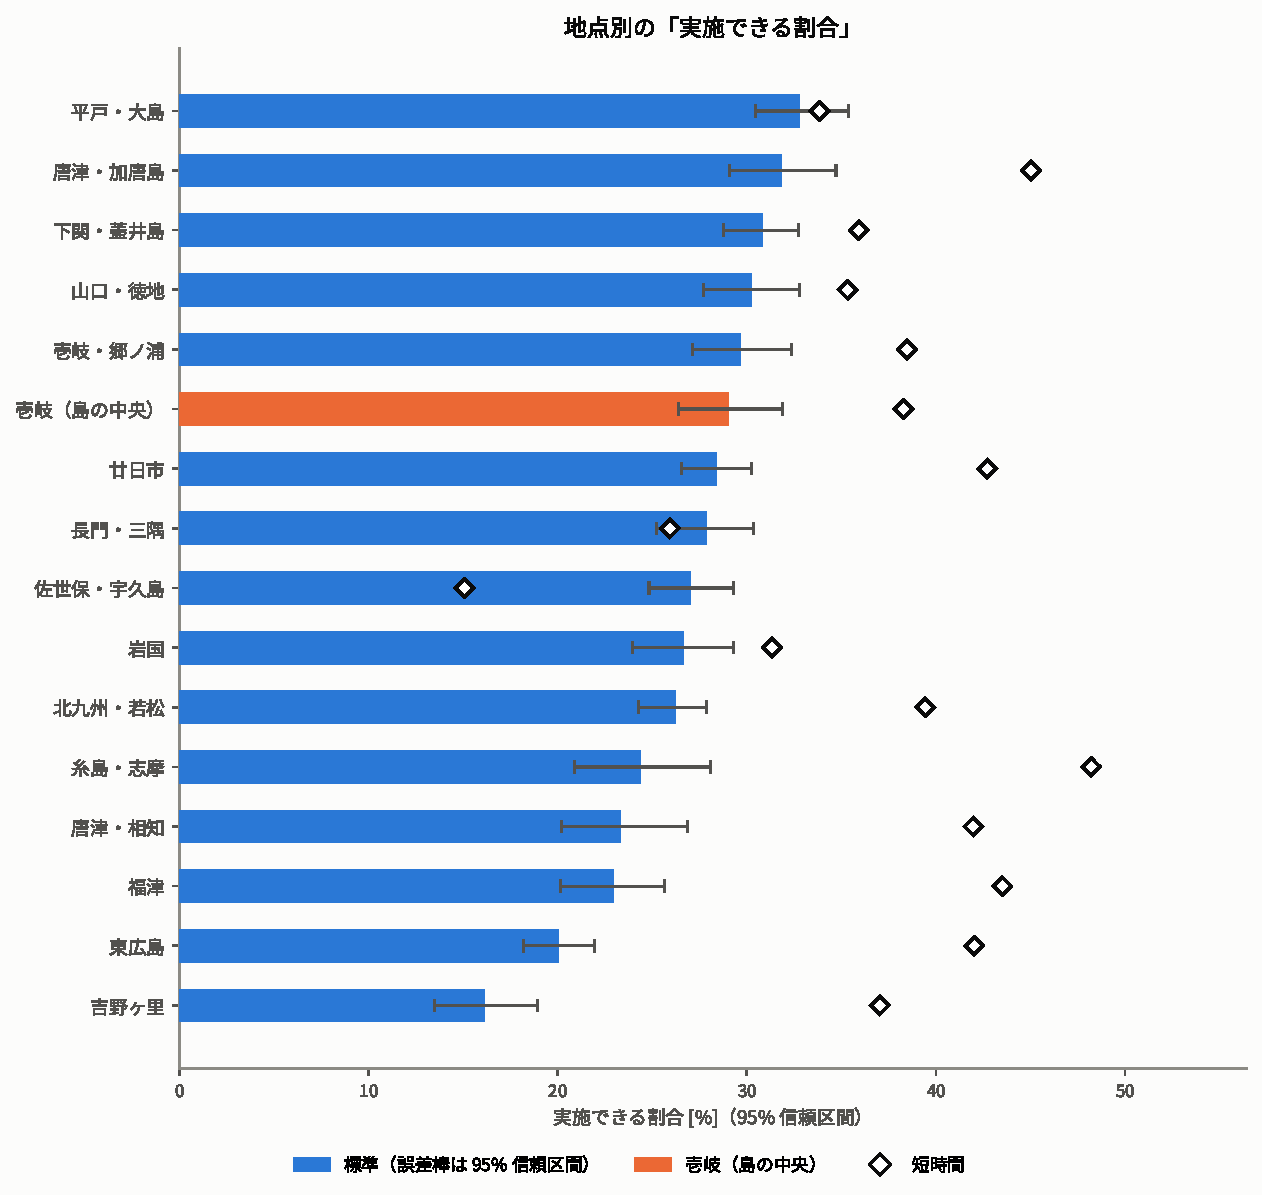
\includegraphics[width=\linewidth]{ranking.pdf}
\caption{実施できる確率の順位（95\% 区間つき）。丸が標準の飛行、四角が短時間の飛行。}
\label{fig:ranking}
\end{figure}

標準の飛行では、平戸・大島（\SI{33}{\percent}）、唐津・加唐島（\SI{32}{\percent}）、
下関・蓋井島（\SI{31}{\percent}）、山口・徳地（\SI{30}{\percent}）、壱岐（\SI{29}{\percent}）が
上位に並ぶ。95\% 区間はおよそ $\pm$\SI{3}{\percent} で、上位 5 地点の差は区間の中に収まる。
つまり標準の飛行では、\textbf{九州北西部から山口県のどこでも、ほぼ同じ 3 割}と考えてよい。
地上気象をアメダスで判定し直すと、壱岐・唐津・平戸はそれぞれ \SIrange{2}{8}{\percent} 上がる（\ref{sec:amedas} 節）。

短時間の飛行では差がはっきりする。糸島・志摩（\SI{48}{\percent}）と唐津・加唐島（\SI{45}{\percent}）が
抜け出し、壱岐（\SI{38}{\percent}）との差は区間の外にある。飛行距離が \SI{180}{\kilo\metre} に縮むと、
糸島や唐津から上げた気球は瀬戸内海の西半分（周防灘・伊予灘）にちょうど落ちる。
ただし落下予測だけを比べると、壱岐（\SI{62}{\percent}）と糸島（\SI{65}{\percent}）の差は小さい。
差の大部分は 9 時の地上気象で、壱岐は \SI{59}{\percent}、糸島は \SI{71}{\percent} の日しか向かない。
地上気象の評価は \ang{0.25} 格子の ERA5 によるもので、島では不確かさが大きい（\ref{sec:amedas} 節）。

\subsection{落下点の散らばり}

図~\ref{fig:clouds} は、上位の地点と壱岐の落下点を 903 日 $\times$ 64 本すべて描いたものである。
落下点は東西に長い帯になり、その帯の半分ほどが瀬戸内海に重なる。成功の大部分は
瀬戸内海への着水で、平野への着地は数 \% にすぎない（図~\ref{fig:breakdown}）。
\textbf{瀬戸内海への着水を認めるかどうかで、結論はほぼ決まる}。認めない場合は
\ref{sec:sensitivity} 節の感度を参照のこと。

\begin{figure}[htbp]
\centering
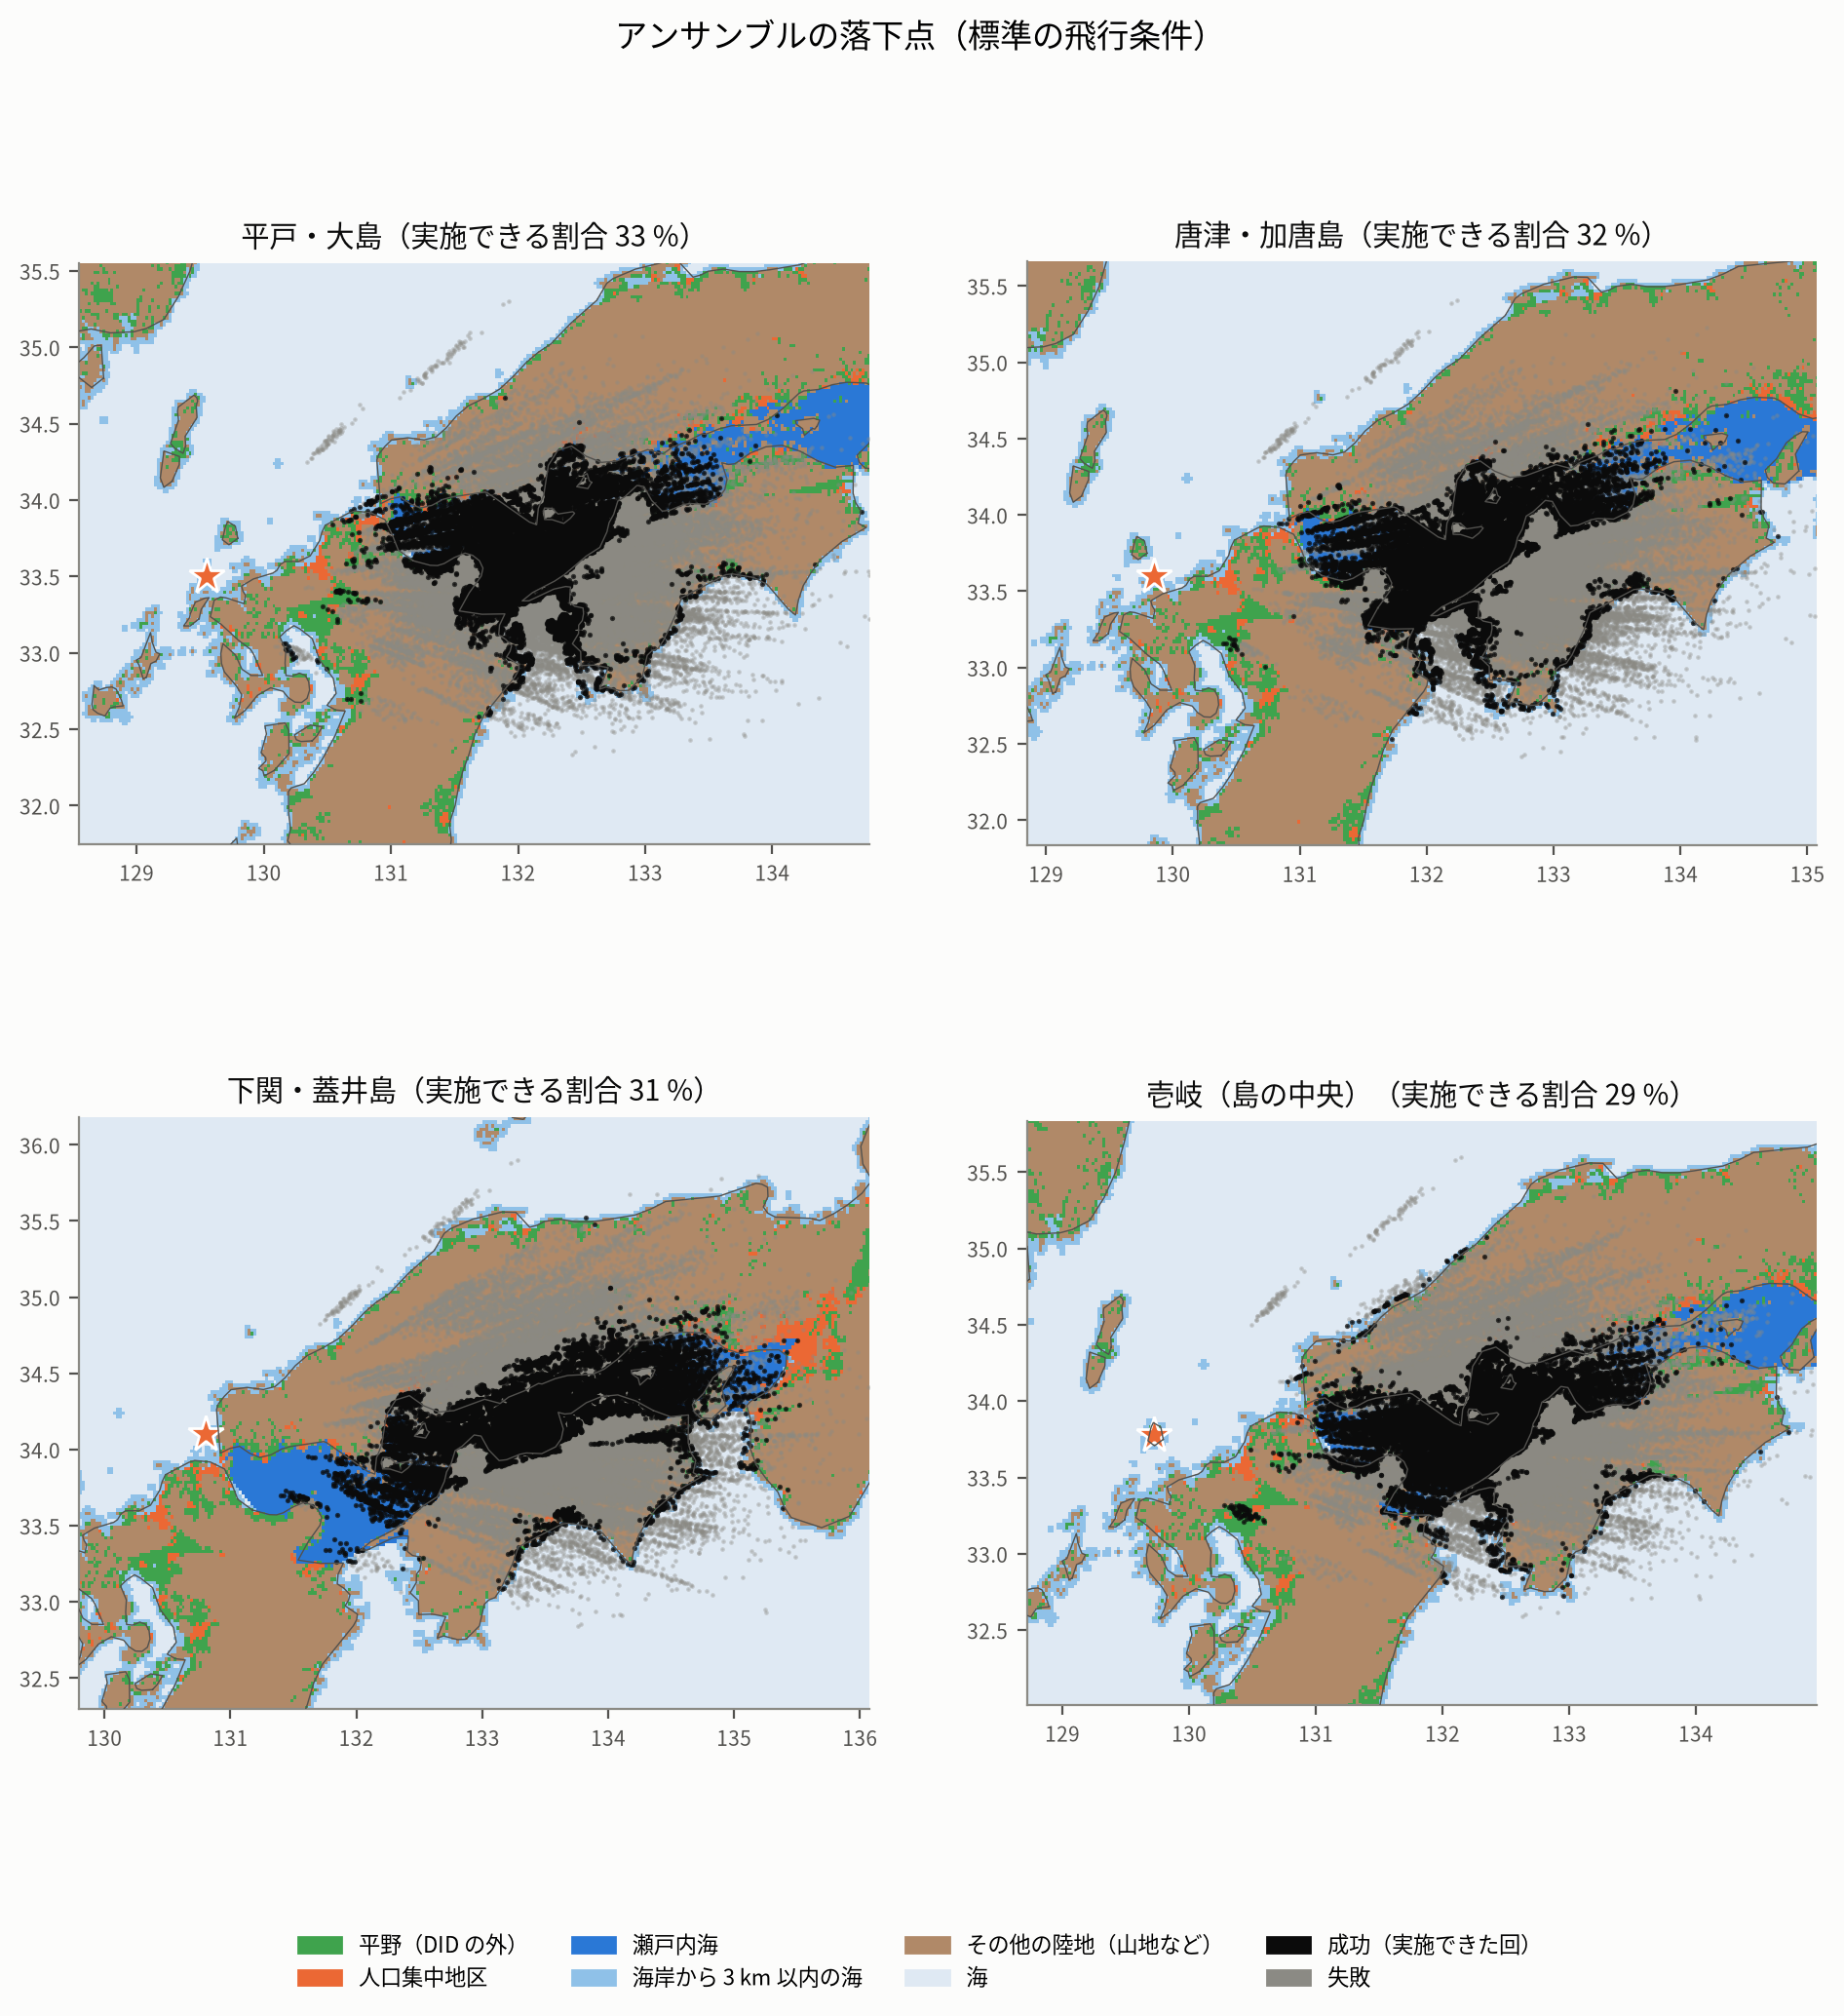
\includegraphics[width=\linewidth]{landing_clouds.png}
\caption{落下点の散らばり（標準の飛行、903 日 $\times$ 64 本）。黒が実施できた回、灰が
それ以外（雪・地上気象で中止の日も含む）。星が打ち上げ地点。各図の題の割合は地上気象を ERA5 で判定した値（壱岐のアメダスでの値は \ref{sec:amedas} 節）。}
\label{fig:clouds}
\end{figure}

\begin{figure}[htbp]
\centering
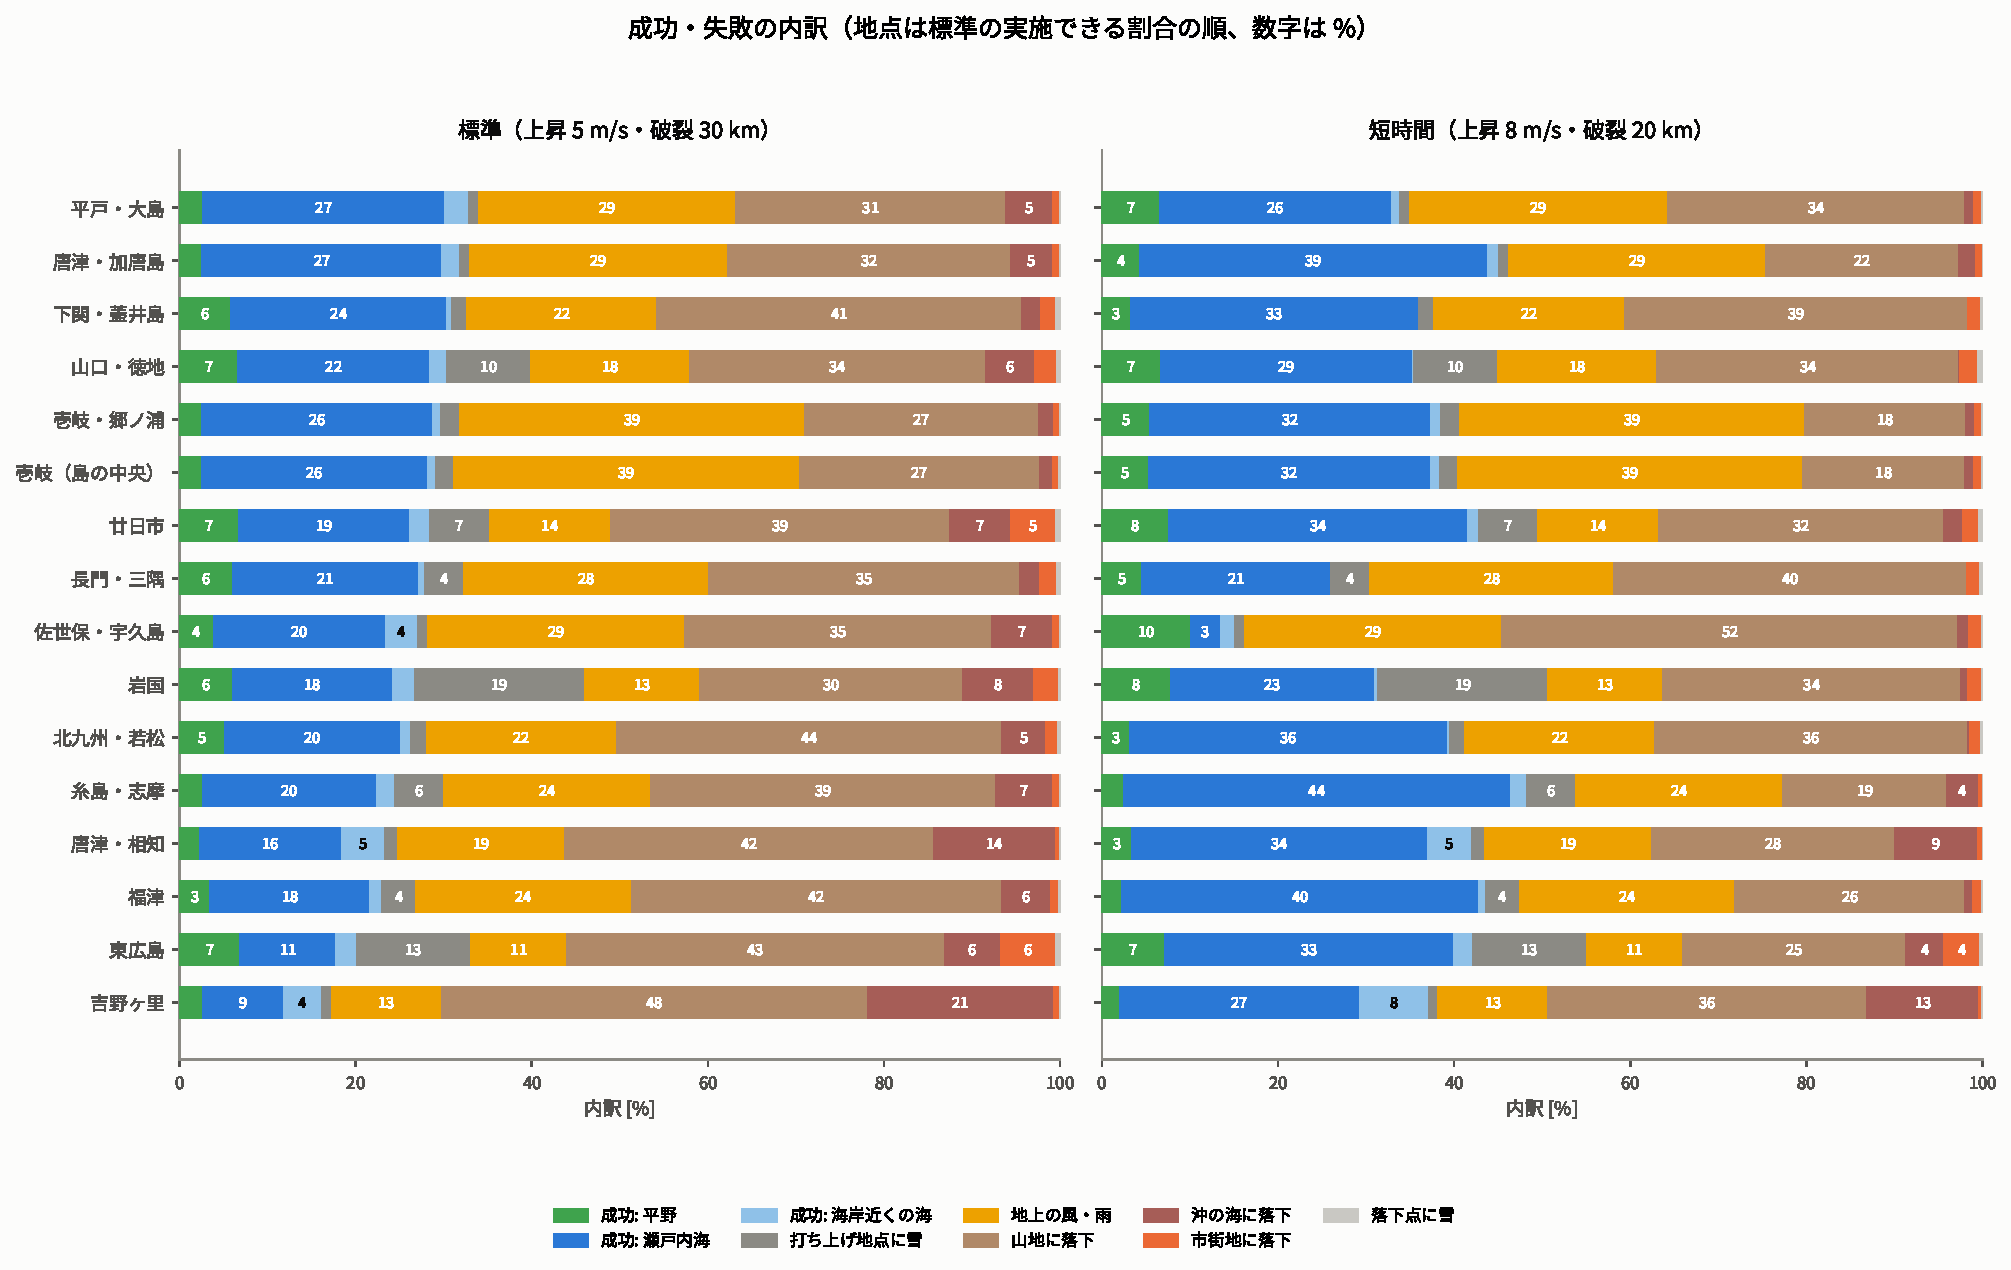
\includegraphics[width=\linewidth]{breakdown.pdf}
\caption{9 時の判断の結果の内訳。左から成功（瀬戸内海・平野・海岸近くの海）、
右へ中止・見送りの理由。雪 → 地上気象 → 落下予測の順に判断したときの割合で、
合計は \SI{100}{\percent}。}
\label{fig:breakdown}
\end{figure}

\subsection{島と本土}

上位には加唐島・蓋井島・平戸の大島・宇久島のような小さな島が入っている。
島は冬でも雪がほとんどなく、地上気象の格子の選び方によっては値が高く出やすい。

実際に機材を運ぶ手間を考えると、近くの本土も比べておく必要がある（格子の値、飛行条件の
ばらつきなし）。
\begin{itemize}
  \item 加唐島の対岸の\textbf{呼子（唐津市、33.55, 129.85）}は標準 \SI{30}{\percent}・
    短時間 \SI{44}{\percent} で、加唐島（32・45）とほとんど変わらない。
  \item 平戸・大島の代わりに\textbf{平戸島}（33.35--33.40, 129.50--129.55）を使うと、
    標準 \SI{30}{\percent}、短時間 \SIrange{23}{29}{\percent} である。
  \item 蓋井島の対岸（下関市吉見付近）は \SIrange{15}{16}{\percent} まで下がる。
    落下予測（\SI{39}{\percent}）は蓋井島（\SI{41}{\percent}）とほぼ同じで、差は地上気象
    （対岸 \SI{39}{\percent}、蓋井島 \SI{77}{\percent}）から来ている。これは両者で参照した ERA5 の
    格子が違うためで、実際の風の差をどこまで表しているかは分からない。
  \item 宗像・福津（33.75--33.85, 130.50--130.60）は標準 \SIrange{20}{26}{\percent}、
    短時間 \SIrange{40}{45}{\percent} で、短時間の飛行なら上位と同等になる。
\end{itemize}

\subsection{打ち上げに使えそうな広場}
\label{sec:osm}

格子の計算で分かるのは「どのあたりから上げるとよいか」までで、実際にどの広場で
上げるかは別に探す必要がある。そこで OpenStreetMap から、壱岐島の全域と、上位の候補地の
半径 \SI{12}{\kilo\metre} 以内（呼子・平戸島・下関の本土側などを含む）にある
公園・グラウンド・競技場・学校の校庭・草地を集めた。

広場ごとに、敷地の中で電線・電柱・建物・鉄塔・林から最も離れられる点を探し、
その距離（ここでは「距離」と呼ぶ）を求めた。面積 \SI{0.3}{\hectare} 以上で、この距離が
\SI{40}{\metre} 以上の所を候補とし、空港の滑走路から \SI{3}{\kilo\metre} 以内は除いた。
同じ学校の敷地とグラウンドのように重なるものは 1 つにまとめた。
さらに、その点から上げたときの実施できる確率を、\ref{sec:method} 節と同じ方法（飛行条件 64 通り、
地上気象は近くにアメダスがあればアメダス）で広場ごとに計算した。

候補は 9 地域で 674 か所あった（表~\ref{tab:spotgroups}、図~\ref{fig:spotswest}）。
同じ地域の中では、確率は広場によってあまり変わらない。たとえば壱岐の 34 か所は、
標準の飛行でどれも \SIrange{36}{38}{\percent} である。場所の良し悪しは地域でほぼ決まり、
地域の中では、電線や建物から離れられるか、使う許可が取れるかで選べばよい。

\begin{table}[htbp]
\centering
\small
\caption{地域ごとの打ち上げ候補地（OpenStreetMap、2026 年 9 月時点）。「距離」は電線・建物・林までの距離。
確率の幅はその地域の候補地の最小〜最大。地上気象は壱岐・平戸・唐津はアメダス、その他は ERA5
（ERA5 は沿岸で確率が低めに出る）。一覧は \texttt{results/launch\_spots.csv}（Google マップのリンクつき）。}
\label{tab:spotgroups}
\resizebox{\linewidth}{!}{\begin{tabular}{lrrccl}
\toprule
地域 & 候補 & 距離 60 m 以上 & 標準 [\%] & 短時間 [\%] & 距離がいちばん大きい所 \\
\midrule
壱岐 & 34 & 10 & 36--38 & 45--50 & 壱岐市立芦辺中学校（110 m） \\
唐津・呼子 & 33 & 20 & 28--35 & 46--51 & （付近: 相賀）（178 m） \\
平戸 & 10 & 6 & 27--34 & 27--35 & 千里ヶ浜鄭成功記念公園（152 m） \\
長門 & 26 & 23 & 23--30 & 20--30 & （付近: 阿武川）（330 m） \\
北九州 & 231 & 188 & 14--28 & 20--42 & 西山公園（698 m） \\
唐津・相知 & 81 & 44 & 19--27 & 37--47 & （付近: 国道202号）（142 m） \\
宗像・福津 & 120 & 103 & 19--27 & 39--45 & （付近: 広陵台五丁目）（512 m） \\
糸島 & 113 & 66 & 20--26 & 39--49 & （名前なし）（237 m） \\
下関 & 26 & 23 & 15--16 & 13--18 & （付近: 豊浦養護学校）（303 m） \\
\bottomrule
\end{tabular}
}
\end{table}

\begin{figure}[htbp]
\centering
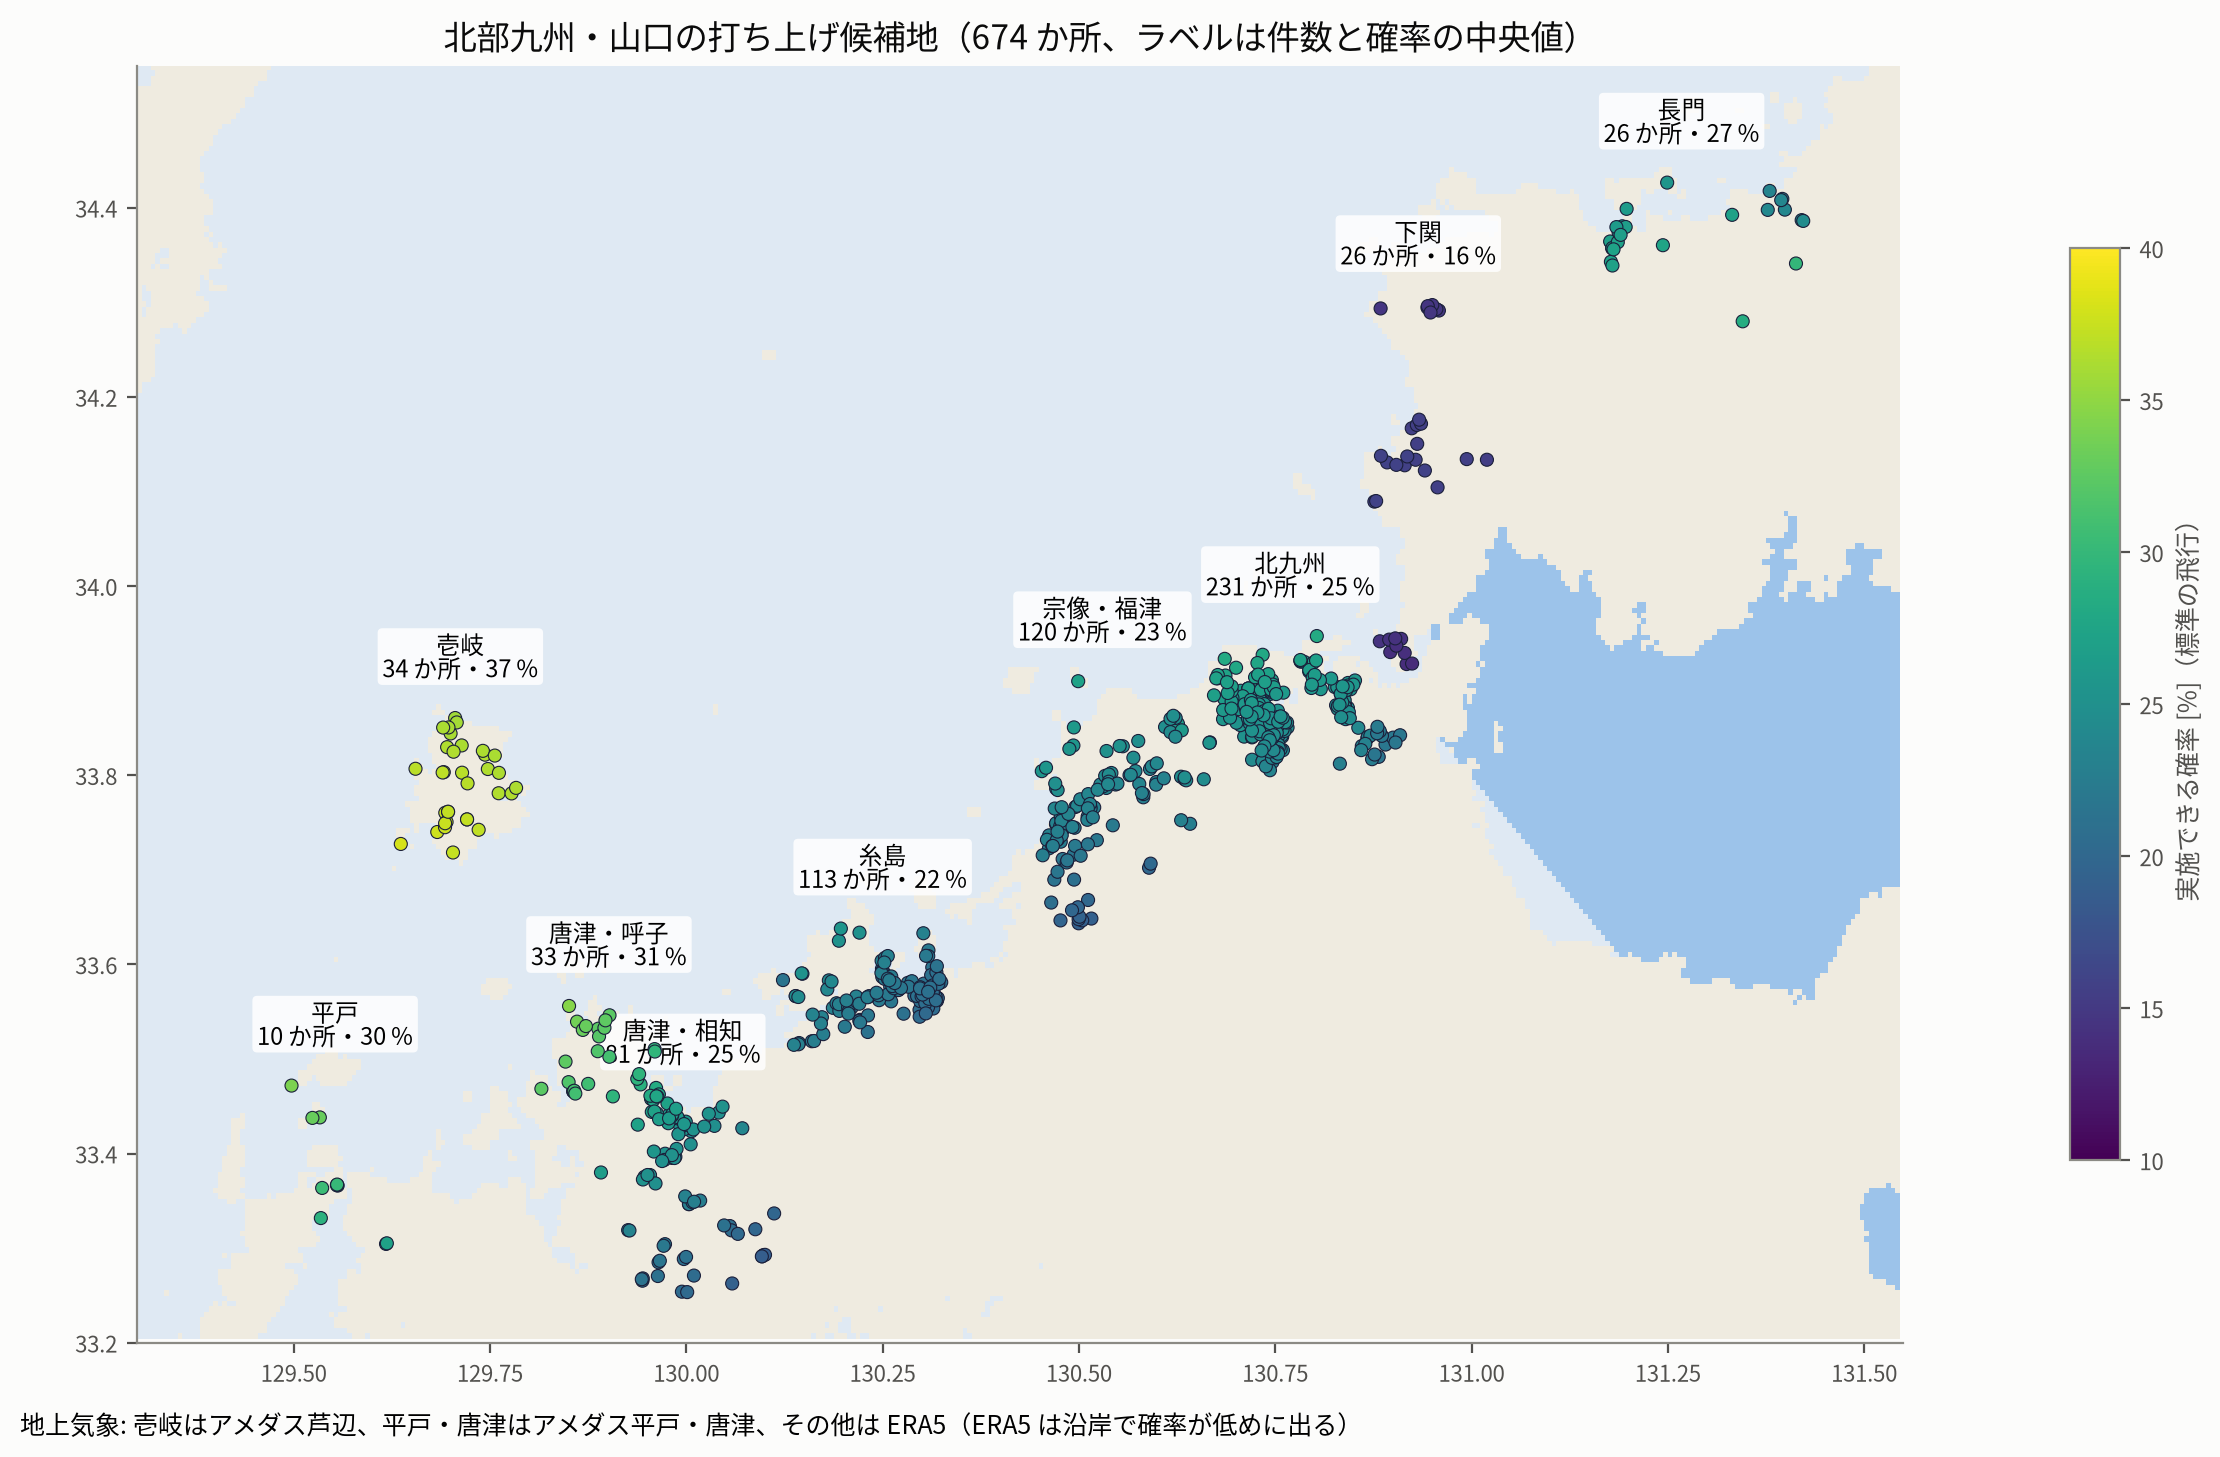
\includegraphics[width=\linewidth]{launch_spots_west.png}
\caption{北部九州・山口の打ち上げ候補地 674 か所。色は標準の飛行で実施できる確率。}
\label{fig:spotswest}
\end{figure}

OpenStreetMap の電線は、地方ではまだ登録が少ない。ここでの「距離」は上限で、実際には
もっと近くに配電線がある可能性が高い。学校の校庭は使用の許可が要る。
一覧は下見の候補を絞るためのもので、使う前に航空写真と現地で電線・建物・立ち入りの可否を
確かめる必要がある。
